\documentclass[10pt]{article}
\usepackage[margin=0.8in]{geometry}
\usepackage[T1]{fontenc}\usepackage{lmodern,graphicx,booktabs,amsmath,amssymb,xcolor,url,float}
\usepackage[colorlinks=true,allcolors=blue]{hyperref}
\setlength{\parskip}{3pt}\setlength{\parindent}{0pt}
\title{When a Verified Answer Does Not Identify a Reusable Correction\\\large A development study of source-bound patches for financial question answering}
\author{OverseeingManyLLMs research prototype}\date{12 September 2026}
\begin{document}\maketitle
\begin{abstract}
A user correcting one answer may hope to improve related work without damaging answers outside the correction's scope. We test a protocol that infers a bounded computation patch from a purchased annotation, checks recipient dependencies and public task constraints, and commits or rolls back the candidate. Two complete development versions use 12 previously inspected TAT-QA source contexts and all 72 original questions, with two common risk-ranked inspections. Neither version produces a supported reusable patch. The refined method and individual correction both achieve 41/72 exact matches, while coarse transfer achieves 43/72 and ordinary reattempts 37/72. Coarse-transfer gains are concentrated in percentage-scale normalization in one context. We therefore do not launch the conditional fresh-context evaluation. Constructed cases verify selective preservation but also expose a harmful formula transfer that passes structural checks. The study identifies missing representation competence and insufficient correction identification, rather than an accuracy advance from correction reuse.
\end{abstract}

\section{Question and closest alternatives}
A question-specific correction certifies an answer, but does not necessarily identify a reusable error cause. Related questions may concern different years, quantities or operations. A preceding experiment in this repository found lower accuracy from adaptive transfer than from risk-ranked individual correction. Here acquisition is fixed so that scope and revision, rather than audit selection, are the intervention under study.

The intended endpoint is additional correct uninspected answers at the same inspection budget, beyond ordinary reattempts and independent source verification. Selective editing is established in SERAC, which explicitly models edit scope and collateral effects \cite{serac}. PAL and Binder already use executable intermediate reasoning \cite{pal,binder}. ExpeL retrieves reusable experience \cite{expel}, and provenance analysis already formalizes dependency preservation \cite{provenance}. Our candidate distinction is a purchased-annotation-to-computation-patch protocol with controlled no-reuse comparisons. Typed records, arithmetic checks and rollback are supporting mechanisms, not separate novelty claims.

\section{Protocol and limited guarantee}
Let $S$ be an immutable table-and-text context and $a_j$ an answer to original question $j$. An optional generated record $r_j$ contains a source hash, source-cell references, operation, operand order, period bindings, scale and expression. Each $x_i$ reads the value of the corresponding recorded cell. The interpreter permits bounded arithmetic only, with at most eight operands, 160 expression characters and 45 syntax-tree nodes. Source binding remains a model hypothesis.

Two question IDs are fixed by the historical risk model and common original answers. An inspection reveals only that question's answer, scale and available derivation, directly replacing that answer. A model continuation attempts a source-supported explanation of the acquired annotation. A difference from the original computation may suggest a local fact-binding, operation/order or scale patch. An already explained annotation remains local. The patch cannot edit source values or consult recipient references.

For candidate $c$ and recipient $j$, define
\[
 C(c,j)=D(c,j)\land P(c,j)\land E(c,j)\land U(c,j),\qquad
 a'_j=\begin{cases}\widehat a_j,&C(c,j),\\a_j,&\text{otherwise}.\end{cases}
\]
Here $D$ checks the implicated dependency, $P$ supported public preconditions, $E$ bounded execution, and $U$ preservation of unaffected bindings. An operation template may generalize across years while preserving recipient operands. A fact-binding replacement requires the actual old reference and must pass the recipient's own period checks. All rejected outputs and inspected answers are preserved by the permitted assignments. Source changes invalidate recorded hashes. These are structural properties, not semantic guarantees. Computation cost is $O(BnK)$ for $B$ inspections, $n$ questions and bounded record size $K$, in addition to explicit source hashing.

\section{Development design and results}
TAT-QA contains financial-report tables and text with human-written benchmark questions \cite{tatqa}. We reuse all 72 questions in 12 training contexts previously used for development, and their saved initial answers. The assignments to agents and two-inspection episodes are constructed. Inspection is ideal annotation disclosure, not observed human supervision. There are 32 arithmetic, 26 span, 12 multi-span and two count annotations. Reliable report identifiers are unavailable, so context pairing is not equivalent to independent-report sampling.

We compare seven methods using common initial outputs, inspections, source access and a structured representation interface. Individual correction changes only inspected answers. Execution evaluates common extracted expressions. Source verification independently rereads never-inspected questions without acquired sibling feedback. Reattempt and coarse transfer regenerate the same broad recipient schedule, respectively without and with disclosures. Constrained patching stages minimal computation changes. Removing recipient-semantic checks is its ablation; donor construction and source/execution checks remain. Different prompts receive fresh continuations. Identical donor requests are cached across patch conditions.

\begin{table}[H]\centering\small
\begin{tabular}{lrrrrr}\toprule
Method & v1 EM & v2 EM & v2 F1 & Repairs/harms & Extra calls\\\midrule
Individual correction & 41 & 41 & 0.611 & 0/0 & 0 \\
Execution only & 41 & 41 & 0.611 & 0/0 & 0 \\
Ordinary reattempt & 42 & 37 & 0.568 & 0/4 & 108 \\
Source verification & 41 & 41 & 0.611 & 0/0 & 48 \\
Coarse transfer & 44 & 43 & 0.636 & 2/0 & 108 \\
Constrained patch & 41 & 41 & 0.611 & 0/0 & 24 \\
No applicability & 41 & 41 & 0.611 & 0/0 & 24 \\
\bottomrule
\end{tabular}
\caption{Development only, 72 original questions and 12 reused source contexts per version. EM columns count correct answers; F1 is a mean. Repairs/harms concern final never-inspected answers in v2. Extra calls exclude the 72 common representation extractions. Versions are not independent replicas.}\label{tab:results}
\end{table}

Every method begins at 20/72 EM. Direct inspection adds 21 correct answers. Patching produces no committed transfer, leaving 41/72, with joint answer/scale correctness 39/72. No v2 method completes a whole context correctly. Final answers remain nonempty even where representations fail. This distinction prevents auxiliary-schema errors from being confused with missing answers.

\begin{figure}[tbp]\centering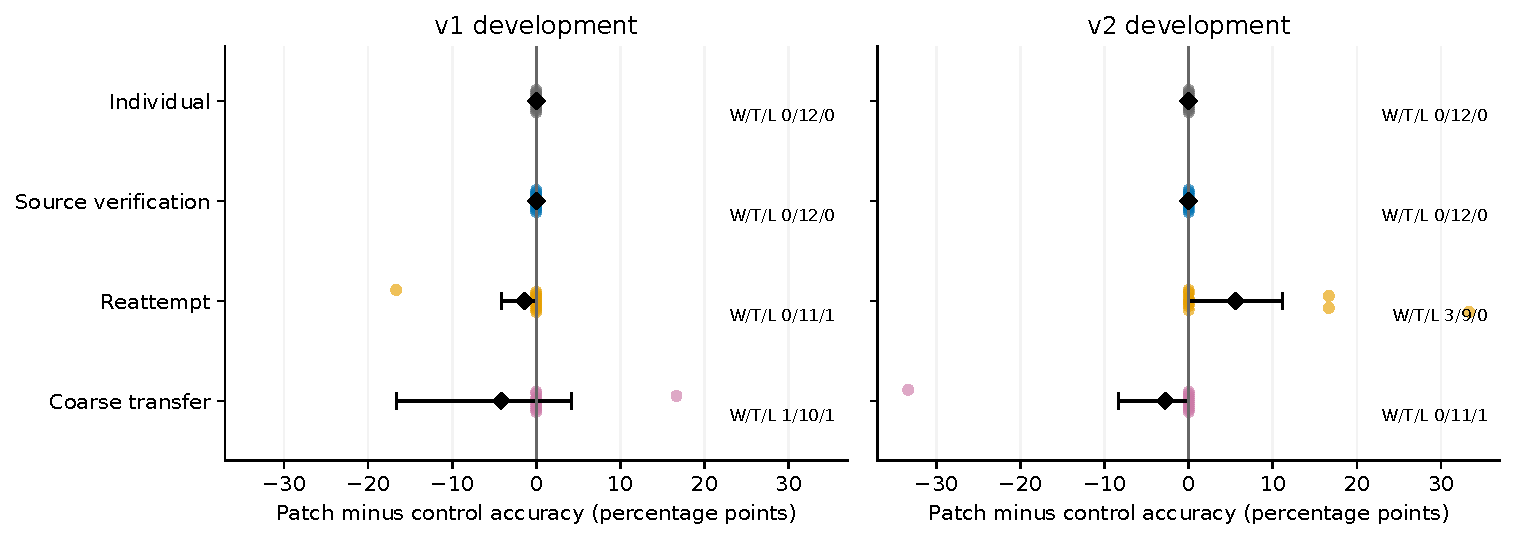
\includegraphics[width=\linewidth]{../../artifacts/correction_applicability/figures/paired_contexts.pdf}
\caption{Generated outputs scored against benchmark annotations. Points are source-context differences; diamonds and bars show means and descriptive 95\% intervals from 2000 paired bootstrap resamples. Positive favors patching. W/T/L counts concern 12 contexts per version. Zero intervals are mechanical equality of retained outputs, not population equivalence.}\label{fig:pairs}
\end{figure}

In v2, patch minus reattempt is +5.56 percentage points, interval [0.00, 11.11], while patch minus coarse transfer is -2.78, interval [-8.33, 0.00]. Its advantage over reattempt is entirely avoidance of regeneration, not correction reuse. Individual correction delivers identical accuracy without patch-generation cost. These are development descriptions and do not establish an independently evaluated improvement.

\section{Coverage, attribution and the gate}
The first version generated 30 executable records, but none passed its public contract. A uniform refinement derived row/section and explicit year metadata from selected cells and simplified the generated schema. It reduced context failures, but only eight v2 records executed and one passed the public contract. Sixty-one outputs had no supported representation. Of 24 inspected donor pairs, 19 lacked complete before/after records and five failed numeric-cell, period or percentage-formula checks. Both versions inferred zero reusable patches.

\begin{figure}[tbp]\centering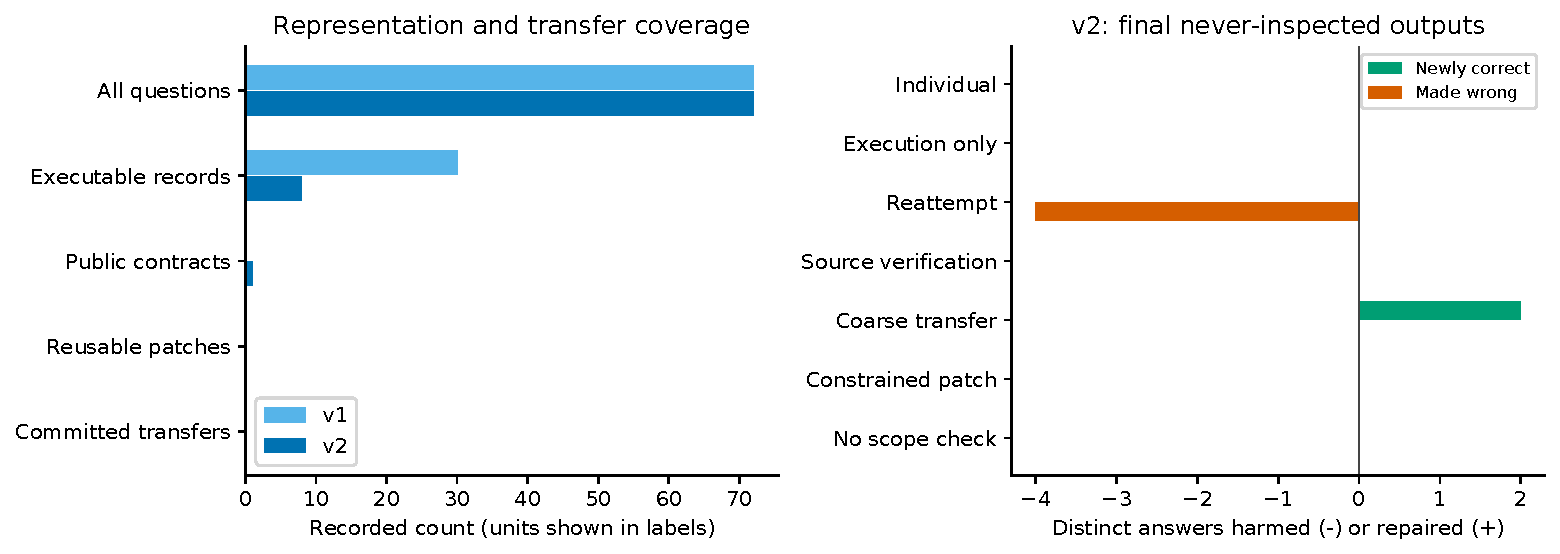
\includegraphics[width=\linewidth]{../../artifacts/correction_applicability/figures/coverage_and_transfer.pdf}
\caption{Recorded development coverage and final never-inspected changes. The funnel has 72 questions, 24 donor disclosures and 108 recipient decisions per version. Those denominators differ. There are 48 never-inspected questions in 12 dependent source groups. Generated representations, simulated inspections and annotated correctness are separate quantities.}\label{fig:coverage}
\end{figure}

Because the recipient-check ablation also receives no supported patches, its tie cannot validate applicability. A post hoc metadata-only pass over the original v1 cell hypotheses admits 12 contracts, diagnosing an interface contribution without replacing v1 results. The later schema guard changes two rejection explanations but no requests, snapshots or final outputs in saved-output replay. All original versions and failures remain preserved.

All final coarse-transfer gains were scale-only changes in one source: four answers in v1 and two in v2. Its table already labels year columns with percent signs. This suggests source-unit interpretation as the closest alternative explanation. One v1 reattempt also fixes a scale error without acquired feedback. The v1 coarse scored harm extends an explanatory span with the requested years. We retain that official EM loss without asserting a new financial falsehood. v2 reattempt adds two thousand-to-million errors and one wrong numeric change, alongside the span mismatch.

The development gate required nontrivial coverage, natural commits, correction-dependent gains and plausible benefit over no-reuse controls. It failed. Although the source audit identified 223 unused technically eligible test contexts, no fresh evaluation was frozen or generated. We did not narrow to favorable questions or introduce a new acquisition algorithm. The implemented conditional protocol is not a demonstrated improvement.

\section{A semantic counterexample}
An acquired example can underdetermine a general operation. Suppose the correct percentage change is $(x_0-x_1)/x_1\times100$. With donor values two and one, the erroneous template $(x_0-x_1)\times100$ fits the annotation. Transferring it to values six and three produces 300\% instead of 100\%. Our structural checks accept this constructed transfer. Therefore neither successful execution nor matching the inspected annotation proves a valid general correction rule. Absolute semantic adequacy remains outside the certificate.

\section{Boundary cases and an inspectable workflow}
Eleven authored cases with 32 controlled perturbation seeds each and two conditions produce 704 CPU-only rows. They cover operation and scale reuse, local facts, wrong periods, missing dependencies, source revisions, failed execution, unrelated outputs and mistaken diagnoses. They do not estimate natural transfer prevalence. Rejection preserves an existing answer, which may remain wrong.

\begin{figure}[tbp]\centering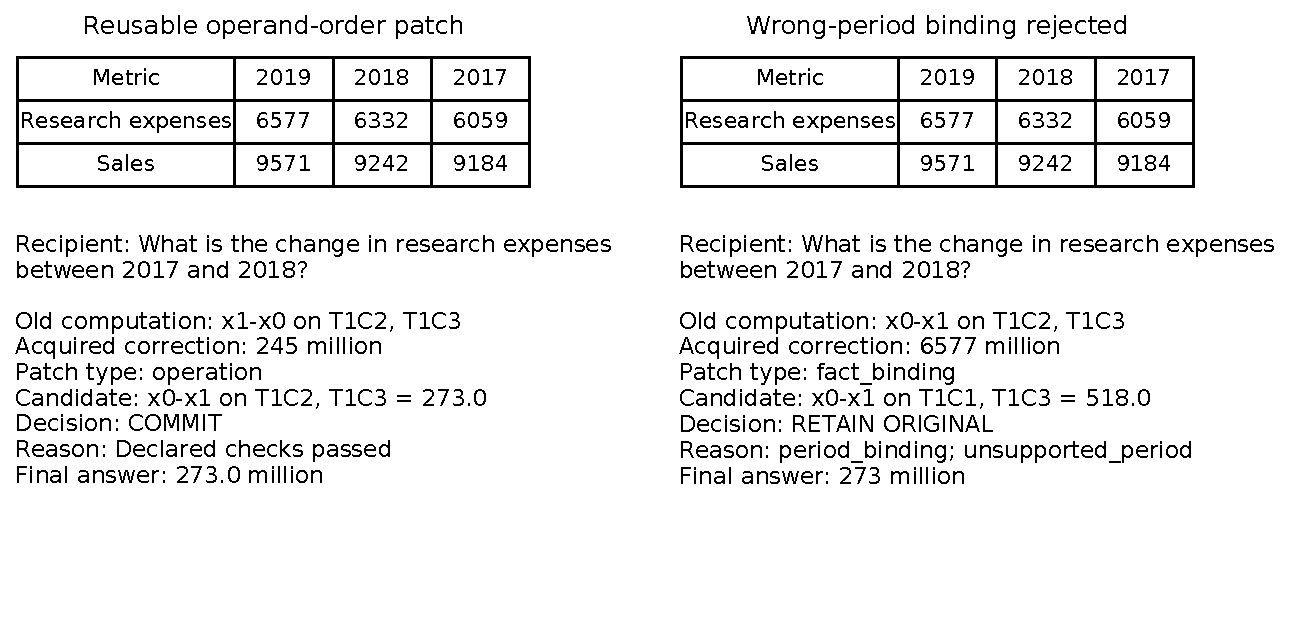
\includegraphics[width=\linewidth]{../../artifacts/correction_applicability/figures/worked_boundaries.pdf}
\caption{Constructed protocol examples using the expense pattern from the historical source audit. Amounts are millions. Left: the acquired operand-order correction changes another period's computation while retaining its cells. Right: a local fact replacement would create an inappropriate period comparison and is rejected. These are authored dependency/error cases, not natural successful transfers.}
\end{figure}

The replay desk displays a question-specific correction, its proposed reusable scope, original/candidate computations, retained answers and expandable source evidence. It reveals only completed inspections and refuses a third. Group 6 is the first development source in fixed order with a donor-computation rejection. Group 1 shows the coarse control's scale changes. The interface does not imply a successful empirical patch. Screenshots and recorded displayed-state hashes document scripted software checks, not participant behavior.

\section{Resources, reproducibility and recommendation}
The existing Qwen2.5-7B-Instruct service uses pinned revision \texttt{a09a35458c702b33eeacc393d103063234e8bc28}, BF16 on one RTX 6000 Ada, and zero CPU offloading. Collection made 720 scheduled requests and 702 GPU attempts. Eighteen v1 requests failed context preflight; there were no retries, failed GPU attempts or unparseable returned JSON objects. Auxiliary representation failures remain in all denominators. Usage was 742,352 prompt and 68,457 completion tokens, with 25m 42s summed generation time. The original server and historical clocks were preserved.

All 168 policy traces reproduce from exact requests and recorded disclosures without sibling labels. The package also contains focused boundary tests, 39 passing historical checks, desktop/mobile interface checks, paired tables and six figures in PDF/SVG/PNG. Source-independent inference is not claimed for questions or repeated policy runs. The separate stage ledger reports cumulative wall time, including work beyond the original 36-hour target.

From a clean checkout, run \texttt{bash research/correction\_applicability/reproduce.sh}. The illustrated note builds with \texttt{bash paper/correction\_applicability/build.sh}. Raw source download and new inference are unnecessary for saved-output reproduction.

Risk-ranked individual correction remains the supported practical default. The next useful experiment is a narrow competence study of source-unit and period binding with independent source reading, before testing whether acquired feedback adds information. This study contributes a falsifiable protocol, transparent gate failure and semantic counterexample. It does not support making constrained correction transfer the paper's central accuracy claim.

\bibliographystyle{plain}\bibliography{references}
\end{document}
